\def\baselinestretch{1}
\chapter{CONCLUSION AND FURTHER WORK}
\label{chap:con}
\graphicspath{{Conclusions/ConclusionsFigs/EPS/}{Conclusions/ConclusionsFigs/}}


\def\baselinestretch{1.66}

\section{Conclusion}

Physics based methods for synthesizing character animation have attracted much research interest in recent years. 
However, efficient methods for natural looking motion are still out of reach. This is mainly because of the complex structure of body dynamics. 
For physics based methods, the planning and inverse dynamic problems are very challenging. 
Optimization or Data Driven based methods are proposed, but such methods often require prohibitive computational time or extensive motion data that easily runs out of memory.

Taking a different perspective, the underlying question of motor synthesis research is how animals move in a complex and variable environment. This topic is more valuable and interesting, and,  in fact, attracts even more research beyond the computer graphics community. 
Biological and robotic researcher investigated  motor control from a very different perspective, and discovered some more properties which may be more crucial for understanding animal motions than visual properties that are  the  main concern of graphic researchers. 
They have identified the limited neural activity, stability and energy efficiency of motor control.

The current idea from biological science and robotic engineering experience rejects the popular ideas of graphic researchers, because the sensing, computation and actuation systems of real animals are not suitable for optimization or database management. 
Animals in nature must adopt a very different strategy for moving. 
The inspiration from biology and robotic research is an explanation of the complexity of body dynamic. 
The complexity of body dynamics is not to challenge the neural control system, on the contrary, the complexity reflects the sophistication of nature. 
A sophisticate mechanical system may ease the control difficulties of many daily motion tasks. 
The new idea is that in fact most of the motion problems have already been solved by nature.
Evolution has equipped animals with very handy mechanical apparatus, so that many motion tasks can be accomplished without any effort. 
To meet a specific purpose, animals only need to modify basic motion behaviours in a clever way.

These ideas inspired this research, to develop animation methods considering of the biological facts. 
The belief is that if our animation methods follow the biological principle, potentially our characters in the virtual world will move and react in a more natural manner. Such a goal has been partly achieved in this research.  
In addition, more valuable results arise from this process. 
To develop simulation programs, intuitive biological ideas are tested for their computational efficiency and logical soundness. 
As a consequence, a new mathematical interpretation and many algorithms are proposed in this research. 
The new idea proposes more detailed information about the motor control process. 
These new ideas are summarized as the Motor Invariant Theory. The new theory is more detailed and accurate compared with current biological ideas, and is applicable to controlling real robotics. 
If it can be proved by further biological research and experiment, this theory may have significant meaning.

Motor Invariant Theory is composed of several interconnecting ideas. 
The theory unifies these ideas in a very different perspective of dynamics. 
The traditional force -motion perspective is not insightful for understanding natural dynamics, because it provides little information about the stability and energy efficiency of motion. 

Motor Invariant Theory adopts the geometrical perspective. 
The concept of phase space is introduced and the dynamic system is transformed into a geometrical structure: the phase portrait. 
After this transformation, motion dynamics can be studied with many geometrical tools. 
On a phase plot, the dynamic system is divided into different regions. 
There is an attractor in each region which attracts all the states in the surrounding states toward it. 
Motor Invariant Theory proposes that animal motion utilizes these attractors for motor control. 
Because attractors promise stability and energy efficiency, they will greatly reduce control difficulties.
 
This idea has support from biological research. 
The idea of organized motions in blocks is proposed  as the motion primitive hypothesis. 
And the idea of utilizing attractors has been proposed by  the equilibrium point hypothesis. 
Such ideas may be new for graphic researchers, but the principles are long established in biological research.


The novelty of Motor Invariant Theory is the idea of the adaptation mechanism. 
Given that the attractors are the starting point for motion planning, the following question is how the neural control system tweaks the dynamics to achieve specific motions. 
During this process, the challenge is that stability must be maintained, energy cost must be minimized and the computation should not last long. 
Optimization based methods are not suitable.  
Also the tracking controllers are not appropriate for motor control, because motions vary greatly.
People walk with different gaits in different situations. 
The idea of local stability control that constrains the motion within a small error range from the reference will make motion lack variation.  Motor Invariant Theory proposes that the stability property should be controlled qualitatively. 
Large deviations from the reference should be allowed while stability is controlled. 
In the geometrical perspective, this means the shape and position of the attractor does not matter, the controller only needs to maintain the attractor and the current state within the basin of attraction. 
This idea is modelled by the mathematical language of topology. 
Maintaining the attractor without considering the shape and position means  the topology remained the same. 
In motor invariant theory, changing the shape and position of attractors is not only allowed but utilized as a powerful tool.  
The idea of changing the shape and position of the attractors not only generates adaptive motions, but also promises stability and energy efficiency and computation efficiency. 
Two methods have been developed following this principle. 
The first idea is entrainment. 
This idea applies to almost all the periodic system. 
For entrainment systems, the periodic behaviour will be enhanced and perturbations are rejected. 
From the geometrical perspective, the entrainment will maintain the topology of limit cycle and enlarge the basin of attraction. 
In addition, the idea of entrainment is well supported by biological research.  
Also the method is computationally efficient.
Another method is based on symmetry and the preserving law of mechanical systems. 
Natural dynamic systems tend to preserve many properties during motion, like energy or momentum. 
Transforming motions in a way that preserves such invariant properties will promise energy efficiently.
Such transformation actions form another important mathematical structure, the Lie group.


It is easy to prove that a Lie group transformation will not alter the topology, thus the stability of transformed motions is guaranteed. 
This provides animators with a direct method for modifying the motion without concerns about stability.  
Also this method is easy to use. 
Because Lie group transformation can be parameterized with a few parameters. 
Animators can modify motions by specifying very few parameters of Lie group, instead of each \dof of the character. 
As examples, three Lie groups are developed, the offset group which  changes the locator positions, which changes the direction of motion; the time scaling group which modifies the speed of motion, and also the energy scaling group which modifies the energy of motion. With such tools, given a motion primitive, animators are allowed to modify the position, speed and amplitude of motion, without worry about the stability. 
As for the computation cost, this research found that for rigid body systems, control input of each group element has a close form formula, and the computational cost is trivial to compute. 
The idea of Lie Group is also supported by biological research, which found that the motion trajectory has many transformation invariant properties.


Because the {\cpg} entrainment and Lie Group transformation are based on the topological invariant principles, these two controllers can be combined.
Such operations will change the shape and location of the locator, resulting in many types of variations in motion. 
If the basin of attraction is modified to capture the current state, the current motion primitive can be maintained. 
However, there are also important applications for changing the shape and position of the locator to avoid current state. 
As a result, the motion will diverge, and finally converge to a different attractor. 
An immediate application is to generate motion failure, which will be useful in many situations. 
The more important application is in motion transition. 
We can tweak the neighbour attractor to capture the current state, which will generate stable transitional motion. 
This shows how motor invariant theory can be easily extended to explain more natural motion phenomena.

Such methods have been applied to control various mechanical systems and characters. 
The bouncing ball example shows how the entrainment forms an attractive limit cycle and how group action changes the shape. 
In this process the bouncing height is maintained and can be justified against many perturbations. 
Another example is bipedal walking.  
Although bipedal walking seems difficult to control,  it can happen naturally because a limit cycle exists.
With the entrainment method, the periodic behaviour is enhanced and the basin of attraction is enlarged.  
This makes passive walking more stable. 
This qualitative control approach can generate different gaits with different body structures and environment conditions. 
When Lie group actions are applied, the passive walker is capable of walking on different terrains (offset action), at different speeds (time scaling) or with different step sizes (energy scaling). 
For the balancing motion primitive, entrainment will turn the dynamic system attractive and group operators will adjust the size of basin of attraction and the time needed to stabilize. 
Also the transitional motion of walking and balance can be synthesized with an energy efficient method requiring little control effort. 

Such simulation results are compared with real life data and they comply with the observed facts. 

This research provides an answer to the way animals achieve computational efficiency, energy efficiency and stability against various perturbations, Motor Invariant Theory proposes a feasible answer.
 For animation researchers, motor invariant theory proposes a method that generates adaptive and natural looking motions in a computationally efficient and reliable way.

But as a new theory, there are still many unanswered questions. 
Finding the attractors in a high dimension dynamic system is not an easy task. 
At the end of the research, several methods are proposed to simplify the dynamic space to make the task of finding locators easier. 
We propose neglecting degrees of freedom in minor motions; dynamic space can be reduced according to the symmetrical properties or exploring the similarity and time shift properties in many mechanical structures. 
Such methods help to add more detail to the synthesized motion, like the rotation, body and arm swing motions. 
Also the method can be extended for more applications like crowd and swimming simulation. 
But this question is not answered completely in this research.

Nature seems to outsmart us. Even though we have learned a lot from nature,  we still have much to learn.



 




\section{Further Work}
Motor Invariant Theory is not an improvement on existing \cms techniques, it is a different paradigm.
This thesis does not explore the full implication and potential of this new theory.
There is room for improvement, new techniques to be developed and even new questions to be answered.
This section summarizes several potential topics that may interest computer graphic  or biological research communities.

\subsection{Stable Templates Of Motion Primitives}

This research  started with a unstable system,  where stability is enhanced by adding control effort.
Motor control is a complex task. 
In many cases, it is impossible to model all the control efforts that turn an unstable system into a stable one.


An alternative method is to start from a stable system and modify its shape to match the observation.
Such methods may lose the details of motion but provide better stability and controllability. 
For games or film production, this idea may be important, animators require controllability and stability over physical realism.
For characters performing acrobatics, the characters must not fall even though the dynamic system is unstable in nature.




\subsection{More Types Of Symmetry}
More types of symmetry will generate more types of transformation that can be applied  to adapt motion.
All the group actions adopted in this research are linear transformation group, which are easy to compute.
But the types of transformation are very limited.
Exploring further types of symmetry may provide  different adaptation schemes and may expand the theory to different motion primitives.
\begin{itemize}

\HiItem{Discrete Symmetry Properties}
Bipedal  walking motions is synthesized in this research, an interesting idea is motions for four or more legs be synthesized based on the bipedal walking strategy.

This can be done by exploring another type of symmetry: discrete symmetry.
For dogs, the hind leg and font leg will move in synchronization or in antiphase.




\HiItem{Non-linear Symmetry from Structural Parameter Turning}
Non-linear symmetry preserving transformation will generate more type of adaptation.
Since non-linear transformation is more difficult to find, it remains questionable how a biological system perceives it and applies it to motion adaptation.
However non-linear transformation is suitable for modelling the transformation  resulting from tweaking system parameters.
From the idea of structural stability we know the results of tweaking system parameters are equivalent to having a one-one mapping transformation.
Further research results from non-linear transformation may potentially completely solve the motion re-targeting problem 


\HiItem{Symmetry of Partial Differential System}

All the methods developed are for  ordinary differential equations, which is good enough for rigid body dynamics.
In fact the topological properties and symmetrical properties also apply to partial differential equations.
A Famous example is the Lorenz transformation group and Maxwell equation.

Symmetries of partial differential equations are important for they may extend the control strategy  to control the motion of elastic bodies or locomotions in fluids.
Such motions are more expensive  and are rarely addressed by current \cms methods.


\end{itemize}

To explore more types of symmetry, reformulating the form of equations may ease the task.
Current dynamic equations are based on a fix coordinates frame.
It is helpful to formulate the equations in a coordinate free manner or in the local frame.






\subsection{Transform the Motion Capture Data}
For computer animation, even though methods for simulating high dimensional characters are proposed.
It may be impractical to synthesize all types of motions by procedural methods.
An alternative method is to use dynamic simulation to modify motion capture data, which is well addressed in many research studies in the computer  graphics community.



Based on the idea of topological equivalence, 
motion primitive of different persons or motions of different situations should have the property of topological equivalence.
In state space, there should exist a one-one mapping transformation function.
Motion Data can be converted into the state space and  transformed by one-one mapping.


We can use the low dimensional model to find the one to one mapping relationship, 
which is applied to transform the high dimensional motion capture data.
Potentially, this method may retain the motion details and involves little computational work. 





\subsection{Muscle Actuation}
In the thesis, control effort is applied directly to each \dof of the mechanical system.
In biological research, this process is not so direct.
The neural system generates some chemicals which affect the material properties of muscles, and force is generated as an indirect side effect.


The question of muscle actuation is untouched in this research,
but with further thought, \moit could also provide an alternative idea of muscle action.
If transformation is the reason for applying control effort, the actuation of muscles can be calculated directly from the transformation, without considering the force generated.
From this perspective, muscle actuation can be easier than calculating the forces.


For the simple  mass spring system,
offset can be implemented by changing the rest length parameter $d$.
Speed action can be implemented by changing the stiffness $K$.
and energy scaling can be achieved by adjusting the stiffness $K$ and then restoring it.
 

The reason is transformation can be achieved by two methods, either control effort or by changing the system parameters.

For biological systems, the method of changing parameters  may be better as it will help motor control system get rid of the necessary feedback and computation. 
In fact most control effort in the thesis is potential energy shaping, which only involves  modifying the potential energy.
If muscles are modelled as springs, then potential energy shaping can also be achieved through modifying spring parameters.

The complex muscle structure may provide a mechanism for fine turning the deformation of the phase portrait and  the attractor can be changed into any possible shape.
This idea may provide a conjecture for further biological research.
For graphic research, incorporating muscles in this manner will have no effect on motion synthesis or computational work.
The potential benefit is that the parameters of muscles can affect the skin deformation.



\subsection{Perception based Dynamics}
Motion perception is a high level capacity; it is based upon our object recognition ability and our dynamic reasoning ability.
Many physiological questions in computer graphics may ultimately rely on recognition and perception research in neural science.
The introduction of a motion synthesis method also touches on  the question of dynamic motion perception and encoding problems in intelligence.
The topological equivalence and symmetry may also provide an understanding of the perception problem.

Based on the idea of topology equivalence, the neural system may not need to encode the details of dynamic system, the neural system can form an analogous dynamic systems in our brain which is analogous to the real dynamic systems.
Such model will lack the detailed accuracy, but get the qualitative properties right.

Based on the idea of symmetry, neural system may store some experience and the symmetrical property of dynamics in the memory.
Our brain may verify dynamics by transforming our experience to match our observation.


We are still not sure which method is better, but for our brain, both methods are more practical than forming a symbolic equation solving the differential equations numerically.
Maybe a new dynamic simulator can be designed to test this hypothesis.

A dynamic simulator can be built upon the topology and symmetry property.
Animators can animate by specifying the attractor and the transformation being  applied.
If the hypothesis is true, even though the method will generate physically inaccurate results, the audience will not notice it.

\subsection{Rethink about the uncanny valley}
In \cms research, uncanny valley is a challenging phenomenon of perception at the  central. 
As shown in Figure~\ref{fig:uncannyValley},when the characters  become more and more realistic, there is a big drop in the perception of likeness.
Only over the valley, perception likeness starts to increase;
Currently, little is known about overcoming the phenomenon,
mainly because the mechanism behind such phenomenon is unclear.

At the end of the the thesis, a conjecture is proposed by extending the idea of motor invariant theory.


\begin{figure}[!htbp]
  \begin{center}
      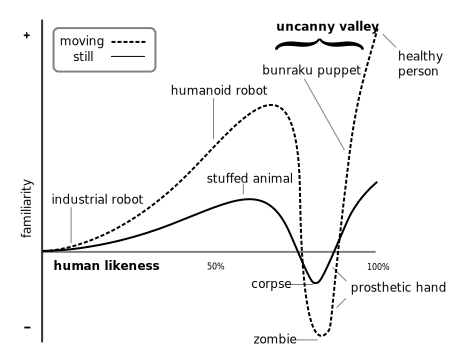
\includegraphics[width=0.5\textwidth]{Mori_Uncanny_Valley}
    \caption{Uncanny Valley}
    \label{fig:uncannyValley}
\end{center}
\end{figure}

The reason behind the uncanny valley is a  a switch of perception mechanism.
For the unfamiliar characters, the perception mechanism is based on analogy,
where the the identification of qualitative properties plays the major role.
As long as the qualitative properties is the the same with our experience, we may accept characters as ``believable''.
In this situation we are checking the Global Motor Invariant.

When the object becomes more familiar, it will trigger our experience memory.
Details are utilized to check the observation against memory,
which closely relate to the idea of Local Motor Invariant.


A object that has desired qualitative property may not have the quantitative details for quantitative perception mechanism.
When the switch of mechanism results in a drop in likeness.
This proposal is bold and early, but might be a worthwhile topic for further biological and physiological research.





%%% ----------------------------------------------------------------------

% ------------------------------------------------------------------------

%%% Local Variables: 
%%% mode: latex
%%% TeX-master: "../thesis"
%%% End: 
